\documentclass[12pt, a4paper, brazil]{article}
\usepackage[utf8]{inputenc}
\usepackage{pslatex}
\usepackage[T1]{fontenc}
\usepackage{amsmath}
\usepackage{pslatex}
\usepackage{amssymb}
\usepackage{graphicx}
\usepackage{graphicx, color}
\usepackage{indentfirst}
\usepackage{setspace}
\fontfamily{times}
\selectfont
\usepackage[top = 3 cm, bottom = 2 cm, left = 2 cm, right = 2 cm]{geometry}
\author{Davi Gabriel de Almeida Dias}
\title{Estrutura de arquivo}
\begin{document}	\begin{center}
	\begin{figure}[!htpb]
		\centering
		
\includegraphics[width=170mm]{logo}
    \vspace{8cm}
	\end{figure}
		{\LARGE \textbf{Entropia de dados em tipos de consoles} \\[3mm]}
		{\large Guilherme Vieira Rodrigues, Davi Gabriel de Almeida Dias e Matheus Madeira}
    \vspace{9cm}
       \\São Paulo\\2023
	\end{center}
	\newpage
    \section*{\Large Sobre o Código}


O codigo faz o calculo da entropia de dados usando como base dados consoles fabricados de 2009 para frente, removemos os dados quantitativos que seriam o preço médio e a data de lançamento e usamos o tipo de console e o fabricante, realizando assim a entropia de duas variantes separadamente.

\onehalfspacing

\section*{\Large Explicação da entropia}
A entropia é uma medida de incerteza ou impureza em um conjunto de dados. Em nossa análise de bases de dados com variáveis qualitativas, calculamos a entropia com base na distribuição de frequência das diferentes categorias da variável.

\vspace{0.5cm}

A fórmula que utilizamos para o cálculo da entropia é a seguinte:

\[
Entropia: - \sum (P(xi) \cdot \log_2(P(xi)))
\]

Onde:

P(xi) representa a proporção de ocorrências da categoria xi em relação ao total de observações.
Para calcular a entropia, seguimos os seguintes passos:

\vspace{0.5cm}

\begin{enumerate}
\item \hspace{0.5cm} Determinamos a frequência de ocorrência de cada categoria.
\item \hspace{0.5cm} Calculamos a proporção de cada categoria, dividindo a frequência pelo total de observações.
\item \hspace{0.5cm} Aplicamos a fórmula da entropia para cada categoria.
\item \hspace{0.5cm} Somamos os resultados de cada categoria para obter a entropia total.
\end{enumerate}

A entropia varia de 0 até um valor máximo, que depende da quantidade de categorias presentes na base de dados. Quanto maior a entropia, maior a incerteza ou impureza nos dados.

No exemplo que mencionou, com a variável ``tipo'' e as categorias ``console de mesa'', ``portátil'' e ``híbrido'', podemos seguir esses passos para calcular a entropia. Utilizando as frequências de ocorrência fornecidas:

\begin{itemize}
  \item \hspace{0.5cm} Coluna ``console de mesa'': 11 ocorrências
  \item \hspace{0.5cm} Coluna ``portátil'': 3 ocorrências
  \item \hspace{0.5cm} Coluna ``híbrido'': 1 ocorrência
\end{itemize}

\newpage

Agora, calculamos a proporção para cada categoria:

\begin{itemize}
  \item \hspace{0.5cm} Proporção da categoria ``console de mesa'': $11/15 = 0.7333$
  \item \hspace{0.5cm} Proporção da categoria ``portátil'': $3/15 = 0.2$
  \item \hspace{0.5cm} Proporção da categoria ``híbrido'': $1/15 = 0.0667$
\end{itemize}

Em seguida, aplicamos a fórmula da entropia para cada categoria:

\begin{itemize}
  \item \hspace{0.5cm} Entropia da categoria ``console de mesa'': $- (0.7333 \log_2(0.7333))$
  \item \hspace{0.5cm} Entropia da categoria ``portátil'': $- (0.2 \log_2(0.2))$
  \item \hspace{0.5cm} Entropia da categoria ``híbrido'': $- (0.0667 \log_2(0.0667))$
\end{itemize}

Por fim, somamos os resultados para obter a entropia total.

\begin{center}
Entropia total = 0.3647 + 0.4644 + 0.1765 = aproximadamente 1.0056.
\end{center}

\begin{itemize}
  \item \hspace{0.5cm} Para calcular a Entropia Máxima consideramos:
  \item \hspace{0.5cm} Entropia máxima = - (3 * (1/3 * log2(1/3)))
  \item \hspace{0.5cm} Entropia máxima = - log2(1/3)
\end{itemize}

Calculando o valor numérico:
\begin{center}
    Entropia máxima = aproximadamente 1.58496
\end{center}

\newpage

\section*{\Large Explicação do código}

O código lê um arquivo CSV chamado consoles.csv usando a biblioteca pandas. Em seguida, conta o número de ocorrências
de cada valor nas colunas tipo e fabricante e calcula a entropia de cada coluna.

A entropia de uma coluna é calculada da seguinte forma:

Calcule a probabilidade de cada valor ocorrer na coluna.
Calcule a entropia da coluna usando a fórmula:
\[
Entropia: - \sum (P(xi) \cdot \log_2(P(xi)))
\]
Por fim, o código imprime a entropia de cada coluna, bem como a entropia máxima que pode ser alcançada para cada coluna.

\begin{figure}[!htpb]
    \centering
    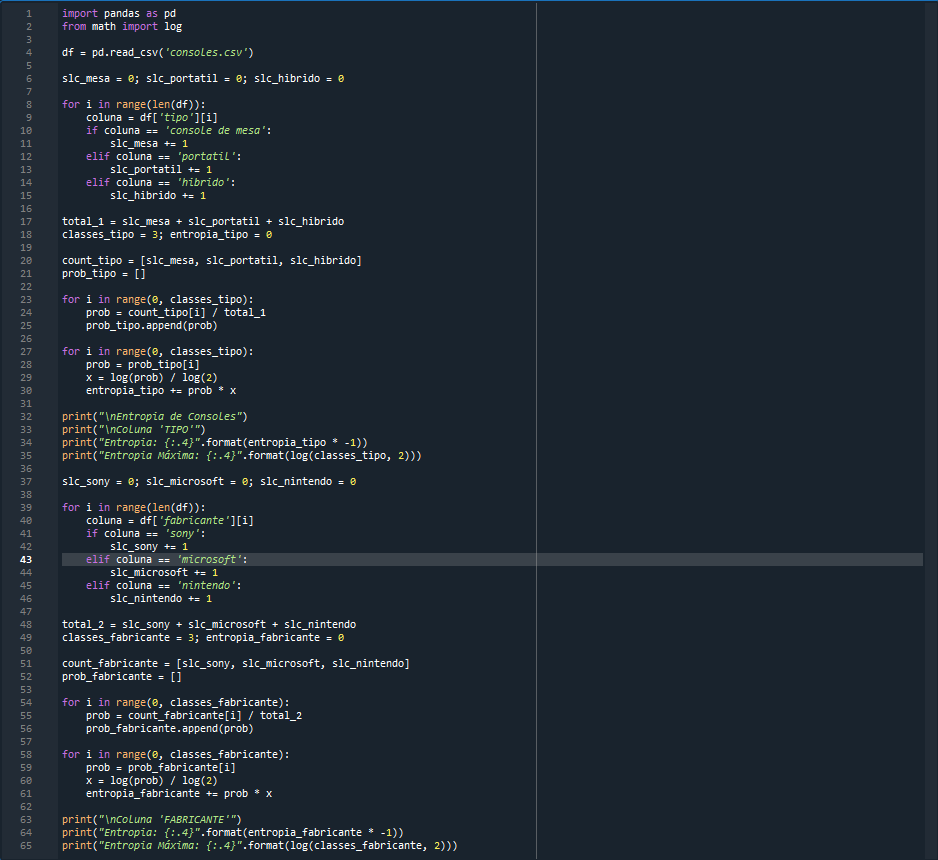
\includegraphics[width=170mm]{code.png}
\end{figure}

\newpage

\section*{\Large Csv}

Um arquivo CSV é um formato de arquivo usado para armazenar dados tabulares, onde os valores são separados por vírgulas. É uma maneira simples e amplamente utilizada de representar informações estruturadas, como tabelas de banco de dados ou planilhas, em um formato de texto legível por máquinas. Cada linha do arquivo CSV representa um registro e os valores são organizados em colunas. O formato CSV é facilmente lido e processado por diferentes aplicativos e linguagens de programação.

\vspace{1cm}

\begin{figure}[!htpb]
    \centering
    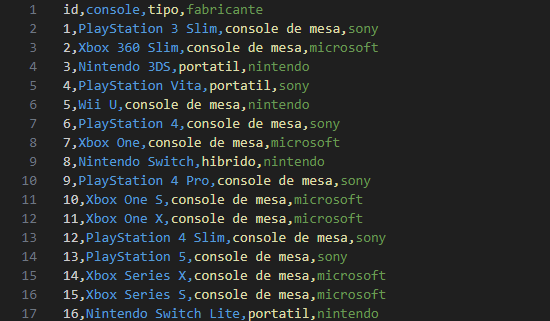
\includegraphics[width=170mm]{CSV.png}
\end{figure}

\end{document}